\begin{activite}[Q.C.M.]
\begin{enumerate}
\item Parmi les nombres suivants, quelles sont les fractions ?
    \begin{colenumerate}{4}
    \item $\dfrac{3}{11}$
    \item $\dfrac{1,2}{1,7}$
    \item $\dfrac{121}{3}$
    \item $\dfrac{3}{0,8}$
    \end{colenumerate}
\item Quels sont les nombres égaux à $\dfrac{2}{5}$ ?
    \begin{colenumerate}{4}
    \item $2,5$
    \item $0,4$
    \item $\dfrac{6}{15}$
    \item $\dfrac{24}{54}$
    \end{colenumerate}
\item Quelles sont les fractions que l'on ne peut plus simplifier ?
    \begin{colenumerate}{4}
    \item $\dfrac{2}{7}$
    \item $\dfrac{120}{55}$
    \item $\dfrac{99}{117}$
    \item$\dfrac{33}{100}$
    \end{colenumerate}
\item  Quels sont les nombres supérieurs à $\dfrac{19}{9}$ ?
    \begin{colenumerate}{4}
    \item $\dfrac{19}{8}$
    \item $\dfrac{22}{9}$
    \item 2
    \item 3
    \end{colenumerate}
\item  Quelle est la somme de $\dfrac{1}{7}$ et $\dfrac{1}{14}$ ?
    \begin{colenumerate}{4}
    \item $\dfrac{11}{714}$
    \item $\dfrac{2}{21}$
    \item $\dfrac{3}{14}$
    \item $\dfrac{3}{7}$
    \end{colenumerate}
\item  Quel est le produit de $\dfrac{8}{9}$ par $\dfrac{3}{4}$ ?
    \begin{colenumerate}{4}
    \item $\dfrac{24}{36}$
    \item $\dfrac{2}{3}$
    \item $\dfrac{32}{27}$
    \item $\dfrac{32 \times 27}{36}$
    \end{colenumerate}
\end{enumerate}
\end{activite}




\begin{activite}[Signes de quotients]
\begin{enumerate}
\item \begin{enumerate}
    \item Calcule les quotients : $(-3) \div 4$ ; $3 \div (-4)$ et $-(3 \div 4)$.
    \item Qu'en déduis-tu pour les nombres $\dfrac{-3}{4}$ ; $\dfrac{3}{-4}$ et $-\dfrac{3}{4}$ ?
\end{enumerate}
\item De la même façon, que dire des nombres $\dfrac{-2,5}{-3,2}$ ; $\dfrac{2,5}{3,2}$ ; $-\dfrac{-2,5}{3,2}$ ; $-\dfrac{2,5}{-3,2}$ ? Justifie.
\item On veut calculer le produit de $\dfrac{-3}{5}$ par $\dfrac{7}{-8}$.

\vspace{1em}
\textbf{1\up{ère} méthode : on détermine d'abord le signe de ce produit.}

    \begin{enumerate}
        \item  Détermine le signe de chacun des deux nombres. Puis déduis, à l'aide de la règle des signes, le signe du produit des deux nombres.
        \item Termine le calcul.
    \end{enumerate}
    
\vspace{1em}
\textbf{2\up{e} méthode : on applique la règle de la multiplication de deux fractions.}
    \begin{enumerate}
        \item Sachant que $\dfrac{-3}{5} \times \dfrac{7}{-8} = \dfrac{(-3)\times 7}{5 \times (-8)}$, calcule le numérateur et le dénominateur du quotient.
        \item Termine le calcul.
    \end{enumerate}
\end{enumerate}
\end{activite}

%%%%%%%%%%%%%%%%%%%%%%%%%%%%%%%%%%%%%%%%%%%%%%%


\begin{activite}[Produits en croix avec tableur]
\begin{enumerate}
\item Écris trois fractions égales à $\dfrac{3}{5}$ autres que $\dfrac{9}{15}$.

Dans un tableur, remplis les cellules comme ci-dessous :

\begin{center}
    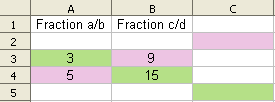
\includegraphics[width=.5\linewidth]{actiTableur}
\end{center}

\item Programme en \texttt{C2} le produit de \texttt{A4} par \texttt{B3} et en \texttt{C5} le produit de \texttt{A3} par \texttt{B4}.
\item Teste dans le tableur les trois fractions trouvées à la question 1. Que remarques-tu dans les cellules \texttt{C2} et \texttt{C5} ?
\item En te servant du tableur, trouve parmi les nombres en écriture fractionnaire suivants ceux qui sont égaux à $\dfrac{3}{5}$ : $\dfrac{301}{501}$ ; $\dfrac{192}{320}$ ; $\dfrac{8,1}{13,5}$ ; $\dfrac{2500}{4000}$.
\item Un nombre en écriture fractionnaire égal à $\dfrac{3}{5}$ s'écrit sous la forme $\dfrac{3\,k}{5\,k}$ où $k$ est un nombre non nul. Démontre que leurs produits en croix sont égaux.
\item On veut déterminer la fraction de dénominateur 120 égale à la fraction $\dfrac{3}{5}$. Remplis les cellules du tableur que l'on connaît et programme en \texttt{B3} le nombre cherché.
\item De la même façon, trouve les nombres manquants : $\dfrac{3}{5}=\dfrac{...}{75}$ ; $\dfrac{3}{5}=\dfrac{...}{125}$ ; $\dfrac{3}{5}=\dfrac{...}{0,25}$.
\end{enumerate}
\end{activite}


%%%%%%%%%%%%%%%%%%%%%%%%%%%%%%%%%%%%%%%%%%%%%%%


\begin{activite}[Inverses]
\begin{enumerate}
\item Quelle est la longueur du côté d'un carré d'aire 1 unité d'aire (U.A.) ?
\item On considère plusieurs rectangles qui ont tous la même aire de 1 U.A.. Recopie puis complète le tableau suivant par les nombres qui conviennent :
 
\renewcommand*\tabularxcolumn[1]{>{\centering\arraybackslash}m{#1}}
\renewcommand{\arraystretch}{1.6}
\begin{CLtableau}{\linewidth}{7}{c}
\hline
& Rectangle 1 & Rectangle 2 & Rectangle 3 & Rectangle 4 & Rectangle 5 & Rectangle 6 \\ \hline
Longueur & 2 & & & 3 & & $\dfrac{4}{3}$ \\ \hline
Largeur & & $0,1$ & $0,25$ & & $\dfrac{1}{7}$ & \\ \hline
\end{CLtableau}

    \begin{enumerate}
        \item Que dire de la longueur de ces rectangles ? Et de la largeur ?
        \item Quel lien y a-t-il entre la longueur et la largeur de ces rectangles ?
        
        \textbf{On dit que deux nombres sont inverses l'un de l'autre quand leur produit est égal à 1.}
        
        \item Recopie et complète : les nombres 2 et ... sont inverses l'un de l'autre, ainsi que $0,1$ et ... ; $0,25$ et ... ; 3 et ... ; $\dfrac{1}{7}$ et ... ; $\dfrac{4}{3}$ et ... .
        
        Que peux-tu dire pour le nombre 1 ?
        
        \item Soit $x$ un nombre non nul, quel est l'inverse de $x$ ? Justifie.
        \item Soient $a$ et $b$ deux nombres non nuls, quel est l'inverse de $\dfrac{a}{b}$ ? Justifie.
    \end{enumerate}
 
\end{enumerate}
\end{activite}



%%%%%%%%%%%%%%%%%%%%%%%%%%%%%%%%%%%%%%%%%%%%%%%



\begin{activite}[Comparaison dans tous les cas]

\begin{partie}[Dénominateurs n'ayant pas de diviseur commun autre que 1]
Corentin le lapin et Luce la puce décident de faire une course. Corentin fait des bonds de $\dfrac{1}{3}$ de mètre tandis que Luce fait des bonds de $\dfrac{1}{5}$ de mètre. 

\begin{center}
    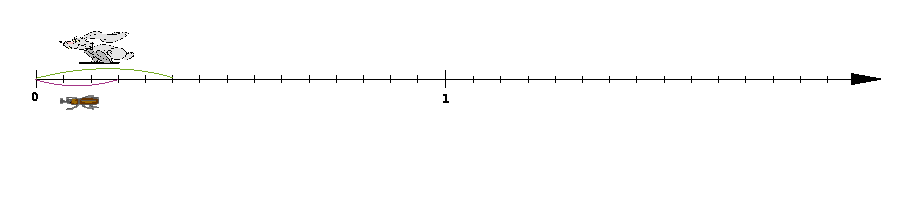
\includegraphics[width=\linewidth]{actiLapinScara}
\end{center}

    \begin{enumerate}
        \item Quand Corentin fait deux bonds, Luce en fait trois. Reproduis la demi-droite graduée ci-dessus représentant la course, puis place les points $C$ et $L$ pour indiquer les positions de Corentin et de Luce.
        \item Complète les phrases suivantes :
        
« Corentin a parcouru $\dfrac{...}{...}$ de mètre, ce qui équivaut à $\dfrac{...}{15}$ de mètre. »

« Luce a parcouru $\dfrac{...}{...}$ de mètre, ce qui équivaut à $\dfrac{...}{15}$ de mètre. »

        \item En t'aidant de la question 2, indique lequel des deux a parcouru la plus grande distance. Parmi les fractions $\dfrac{2}{3}$ et $\dfrac{3}{5}$, laquelle est la plus grande ?
    \end{enumerate}
\end{partie}

\begin{partie}[Dénominateurs ayant plusieurs diviseurs communs]
Lola la tortue et Jeannot le lièvre décident de faire une course sur une demi-droite graduée. Le point de départ est l'origine de la demi-droite. Lola parcourt $\dfrac{5}{4}$ d'unité et Jeannot parcourt $\dfrac{7}{6}$ d'unité.
    \begin{enumerate}
        \item Trace une demi-droite et gradue-la pour y placer les points $L$ et $J$ indiquant les positions de Lola et Jeannot.
        \item Lequel des deux a parcouru le plus grand trajet ? Parmi les fractions $\dfrac{5}{4}$ et $\dfrac{7}{6}$, laquelle est la plus grande ?
    \end{enumerate}
\end{partie}


\begin{partie}[Bilan]
\begin{enumerate}
    \item Énonce une règle qui permet de comparer des fractions de dénominateurs différents.
    \item Applique la règle que tu as trouvée pour comparer : $\dfrac{7}{5}$ et $\dfrac{13}{11}$ puis $\dfrac{3}{25}$ et $\dfrac{1}{10}$.
\end{enumerate}
\end{partie}

\end{activite}

%%%%%%%%%%%%%%%%%%%%%%%%%%%%%%%%%%%%%%%%%%%%%%%


\begin{activite}[Divisions]
\begin{enumerate}
\item Sachant que pour tous nombres $a$ et $b$ non nuls : $\dfrac{a}{b}=a \times \dfrac{1}{b}$, décompose de la même façon le quotient $\dfrac{\dfrac{3}{2}}{\dfrac{5}{3}}$.
\item Que peux-tu dire du nombre $\dfrac{1}{\dfrac{5}{3}}$ ? Déduis-en une fraction égale à ce nombre.
\item Transforme alors le quotient $\dfrac{\dfrac{3}{2}}{\dfrac{5}{3}}$ en produit et complète la phrase suivante : \emph{« Diviser par une fraction, c'est ... .».}
\item Termine alors le calcul du quotient de $\dfrac{3}{2}$ par $\dfrac{5}{3}$.
\item Applique cette règle pour effectuer les calculs suivants : $\dfrac{\dfrac{10}{11}}{\dfrac{7}{8}}$ ; $\dfrac{\dfrac{4}{7}}{\dfrac{5}{9}}$ ; $\dfrac{\dfrac{2}{5}}{\dfrac{14}{3}}$.
\end{enumerate}
\end{activite}
